\chapter{Zat Murni dan Campuran}\label{ch:g6:pure-substances-and-mixtures}

Label sebotol air mineral mencantumkan selusin zat terlarut, lengkap
dengan jumlahnya dalam miligram per liter. Air yang keluar dari alat
pemurni di laboratorium tidak mencantumkan satu pun. Keduanya jernih dan
tak berwarna, keduanya melepas dahaga --- tetapi hanya satu di antaranya
yang oleh ahli kimia disebut murni. Bab ini memberi kata ``murni''
artinya yang tepat, dan menunjukkan cara membedakan \omterm{def:g6:pure-substances-and-mixtures:pure-substance}{zat murni} dari
\omterm{def:g6:pure-substances-and-mixtures:mixture}{campuran} tanpa mencicipi apa pun.

\begin{recall}
\omterm{def:g2:mixing-and-dissolving:mix}{Mencampur} berarti menyatukan benda-benda yang berbeda; padatan yang
\omterm{def:g2:mixing-and-dissolving:dissolve}{larut} dalam air membiarkan cairannya jernih, dan cairan jernih itu
adalah larutan (\cref{ch:g2:mixing-and-dissolving}). \omterm{def:g6:pure-substances-and-mixtures:mixture}{Campuran} dapat
dipisahkan dengan \omterm{def:g3:separating-mixtures:sieve}{pengayakan}, \omterm{def:g3:separating-mixtures:decant}{dekantasi}, \omterm{def:g3:separating-mixtures:filter}{penyaringan}, dan \omterm{def:g3:separating-mixtures:evaporate}{penguapan}
(\cref{ch:g3:separating-mixtures}). Setiap bahan memiliki sifat yang
dapat diuji: keras atau lunak, bening atau tidak, terapung atau
tenggelam (\cref{ch:g1:materials-around-us}).
\end{recall}

\section{Spesies kimia dan zat murni}

\begin{definition}[Spesies kimia]\label{def:g6:pure-substances-and-mixtures:species}
Sebuah \emph{spesies kimia}\index{spesies kimia} adalah satu jenis zat
tertentu, dengan namanya sendiri dan sifat-sifatnya sendiri: air, gula,
garam, oksigen, etanol (alkohol dalam anggur), besi.
\end{definition}

\begin{definition}[Zat murni]\label{def:g6:pure-substances-and-mixtures:pure-substance}
Sebuah \emph{zat murni}\index{zat murni} hanya terdiri atas satu \omterm{def:g6:pure-substances-and-mixtures:species}{spesies
kimia} dan tidak ada yang lain: air suling, sebutir kristal gula, cincin
dari emas murni.
\end{definition}

\begin{definition}[Campuran]\label{def:g6:pure-substances-and-mixtures:mixture}
Sebuah \emph{campuran}\index{campuran} mengandung beberapa \omterm{def:g6:pure-substances-and-mixtures:species}{spesies
kimia}. \omterm{def:g4:air-a-mixture-of-gases:air}{Udara}, air laut, air mineral, susu, granit, dan jus jeruk adalah
campuran.
\end{definition}

\begin{remark}[Murni dalam bahasa sehari-hari]\label{rem:g6:pure-substances-and-mixtures:everyday}
Kotak bertuliskan ``jus jeruk murni'' berarti tidak ada apa pun yang
ditambahkan ke dalam jus itu. Bagi ahli kimia, jus itu tetap \omterm{def:g6:pure-substances-and-mixtures:mixture}{campuran}:
air, gula-gula, asam, vitamin, zat warna, dan zat perisa, banyak \omterm{def:g6:pure-substances-and-mixtures:species}{spesies
kimia}. ``Air pegunungan murni'' pun \omterm{def:g6:pure-substances-and-mixtures:mixture}{campuran}: air dengan garam-garam
terlarut.
\end{remark}

\begin{omfigure}
\begin{tikzpicture}[font=\small, level distance=1.55cm,
    box/.style={draw=omDef, fill=omDef!6, rounded corners=2pt, align=center,
      inner sep=4pt},
    level 1/.style={sibling distance=7.2cm},
    level 2/.style={sibling distance=3.6cm},
    edge from parent/.style={draw, thick, omDef, ->}]
  \node[box] {materi}
    child {node[box] {zat murni\\ \footnotesize satu spesies kimia}
      child {node[box, draw=black!40, fill=white] {air suling,\\ garam, besi}}}
    child {node[box] {campuran\\ \footnotesize beberapa spesies kimia}
      child {node[box] {homogen\\ \footnotesize tampak seragam}
        child {node[box, draw=black!40, fill=white] {air asin,\\ udara}}}
      child {node[box] {heterogen\\ \footnotesize bagiannya terlihat}
        child {node[box, draw=black!40, fill=white] {air berlumpur,\\ granit}}}};
\end{tikzpicture}

{\small Memilah materi. Kotak-kotak paling bawah memberi contoh setiap
jenis.}
\end{omfigure}

\section{Campuran homogen dan heterogen}

\begin{definition}[Campuran homogen dan heterogen]\label{def:g6:pure-substances-and-mixtures:homogeneous}
Sebuah \omterm{def:g6:pure-substances-and-mixtures:mixture}{campuran} disebut \emph{campuran homogen}\index{campuran homogen}
jika bagian-bagiannya yang berbeda tidak dapat dibedakan dengan mata,
bahkan dengan kaca pembesar: \omterm{def:g6:pure-substances-and-mixtures:mixture}{campuran} itu tampak sama di mana-mana.
\omterm{def:g6:pure-substances-and-mixtures:mixture}{Campuran} itu disebut \emph{campuran heterogen}\index{campuran heterogen}
jika sedikitnya dua bagian yang berbeda dapat terlihat.
\end{definition}

\begin{example}[Empat campuran]\label{ex:g6:pure-substances-and-mixtures:four}
Air asin dan \omterm{def:g4:air-a-mixture-of-gases:air}{udara} homogen: bagian-bagiannya tidak terlihat. Minyak di
atas air heterogen: ada dua lapisan. Air berlumpur heterogen:
butiran-butiran melayang di dalamnya lalu mengendap. Jus jeruk dengan
bulir heterogen: serpihan bulirnya terlihat.
\end{example}

\begin{omfigure}
\begin{tikzpicture}[font=\small, scale=1.15]
  \pic[transform shape] at (0,0) {beaker={0.7}{omWater!80}};
  \node[anchor=north, align=center] at (0,-0.15) {air asin:\\ homogen};
  \pic[transform shape] at (2.6,0) {beaker={0.7}{omWater!80}};
  \fill[yellow!55!orange!60] (1.8,1.05) rectangle (3.4,1.4);
  \draw[omGlass, line width=0.7pt] (1.8,1.05) -- (1.8,1.4) (3.4,1.05) -- (3.4,1.4);
  \node[anchor=north, align=center] at (2.6,-0.15) {minyak di atas air:\\ heterogen};
  \pic[transform shape] at (5.2,0) {beaker={0.7}{brown!25}};
  \foreach \x/\y in {4.6/0.3,4.9/0.7,5.3/0.5,5.6/1.0,5.0/1.1,5.4/0.2,5.8/0.6}
    \fill[brown!65] (\x,\y) circle (0.04);
  \fill[brown!60] (4.4,0) rectangle (6.0,0.12);
  \node[anchor=north, align=center] at (5.2,-0.15) {air berlumpur:\\ heterogen};
  \pic[transform shape] at (7.8,0) {beaker={0.7}{orange!45}};
  \foreach \x/\y in {7.3/0.35,7.6/0.8,8.0/0.5,8.3/1.0,7.7/1.15,8.2/0.25,7.45/0.65}
    \fill[orange!80!brown] (\x,\y) ellipse (0.08 and 0.03);
  \node[anchor=north, align=center] at (7.8,-0.15) {jus berbulir:\\ heterogen};
\end{tikzpicture}

{\small Satu \omterm{def:g6:pure-substances-and-mixtures:homogeneous}{campuran homogen} dan tiga \omterm{def:g6:pure-substances-and-mixtures:homogeneous}{campuran heterogen}.}
\end{omfigure}

\begin{omfigure}
\begin{minipage}[b]{0.48\linewidth}\centering
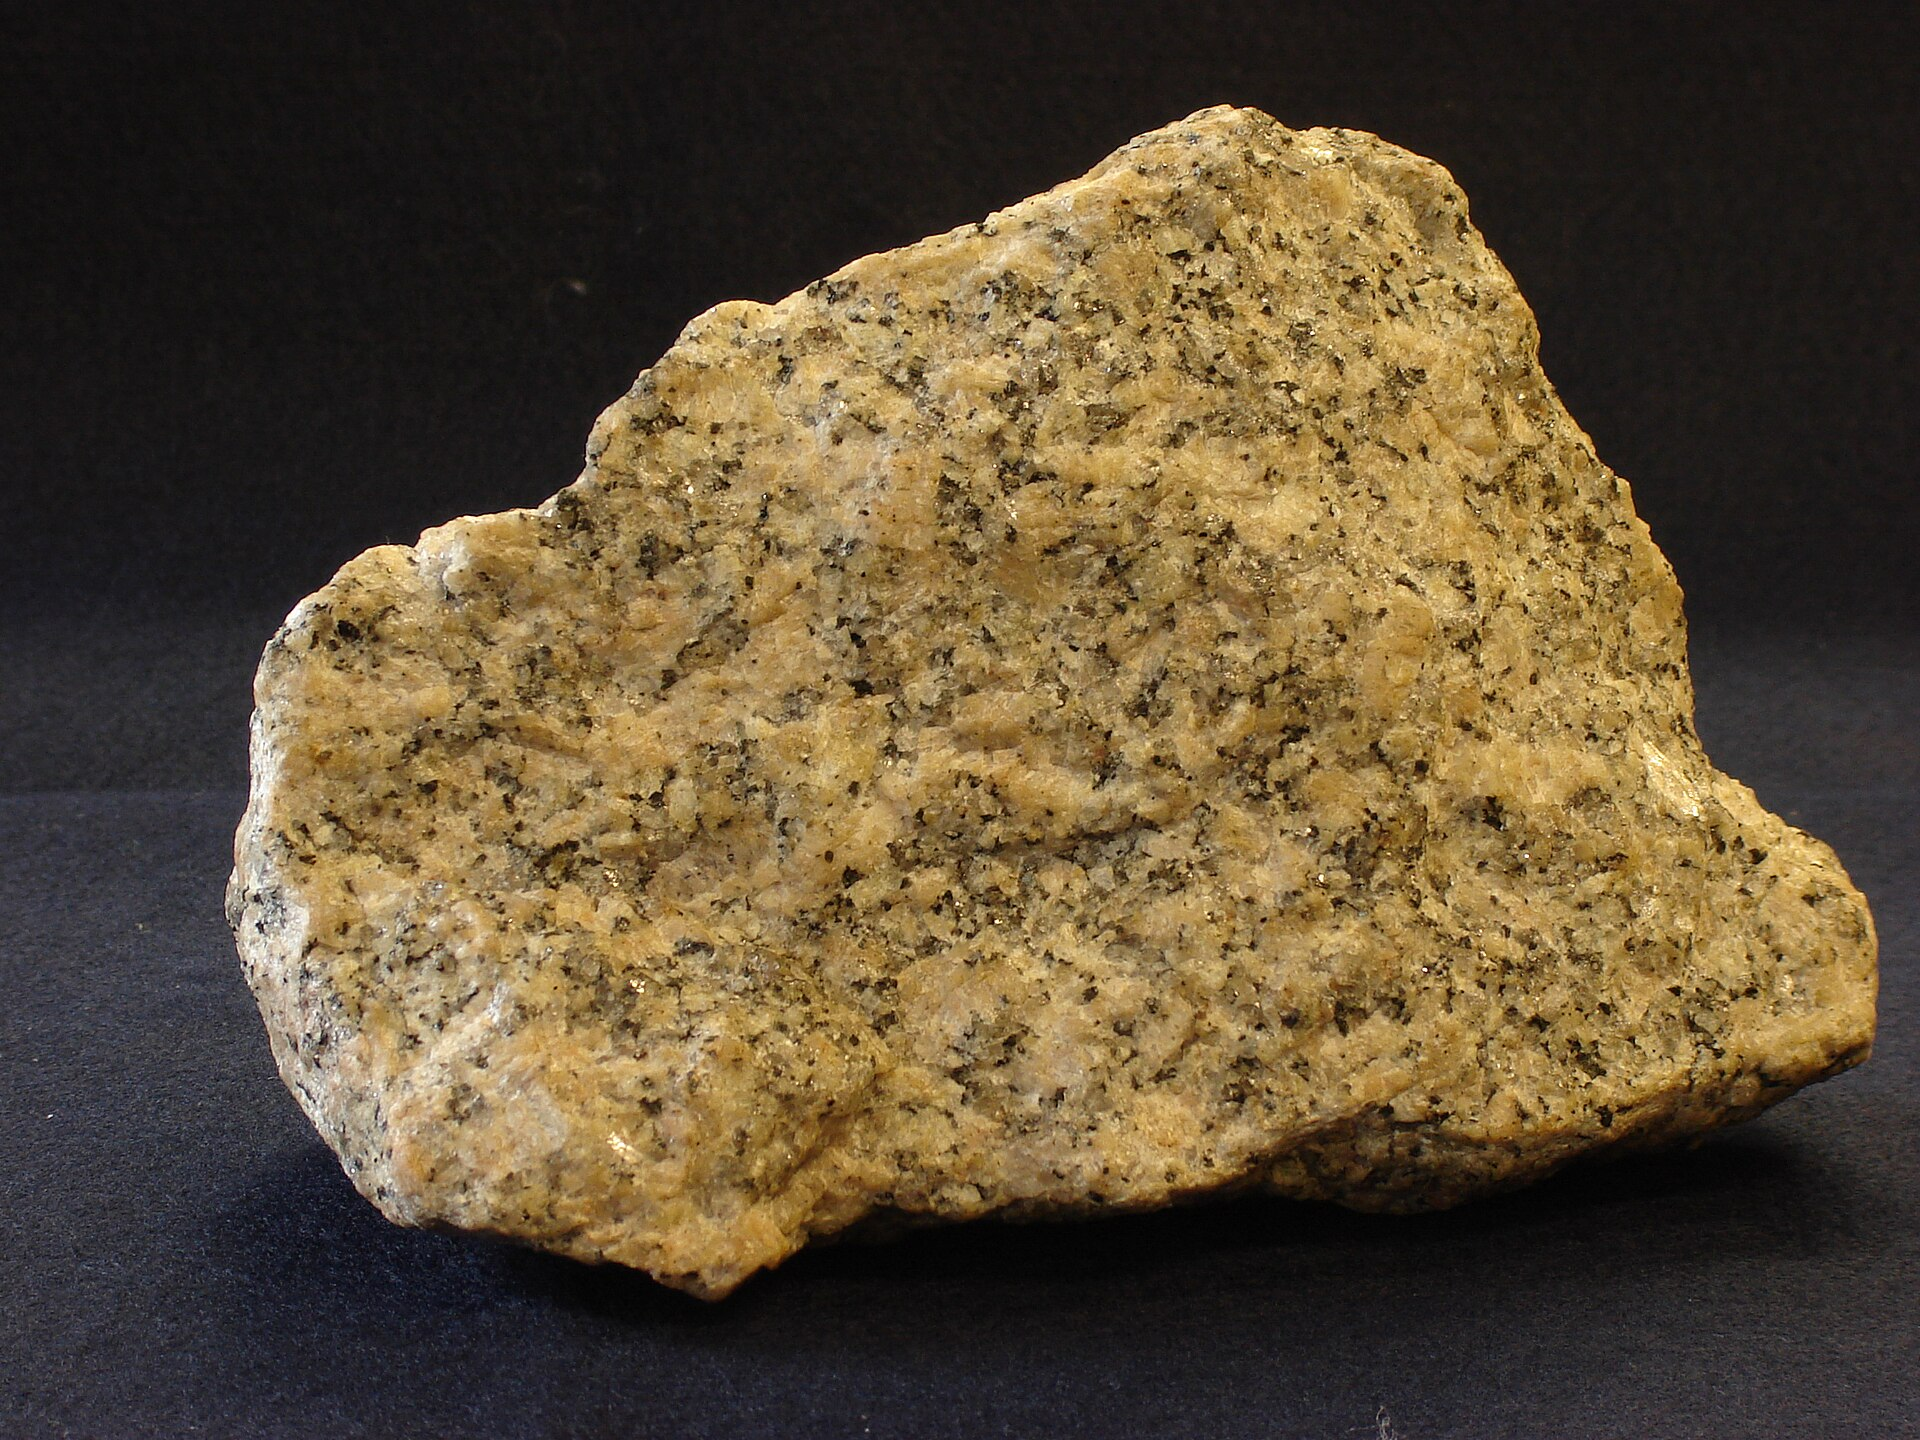
\includegraphics[width=\linewidth,height=4.6cm,keepaspectratio]{images/book1/granite.jpg}

{\small Granit: butiran tiga atau empat mineral yang berbeda dapat
terlihat. Sebuah padatan heterogen. Foto: Eurico Zimbres, CC\ BY-SA\ 2.0\ br.}
\end{minipage}\hfill
\begin{minipage}[b]{0.48\linewidth}\centering
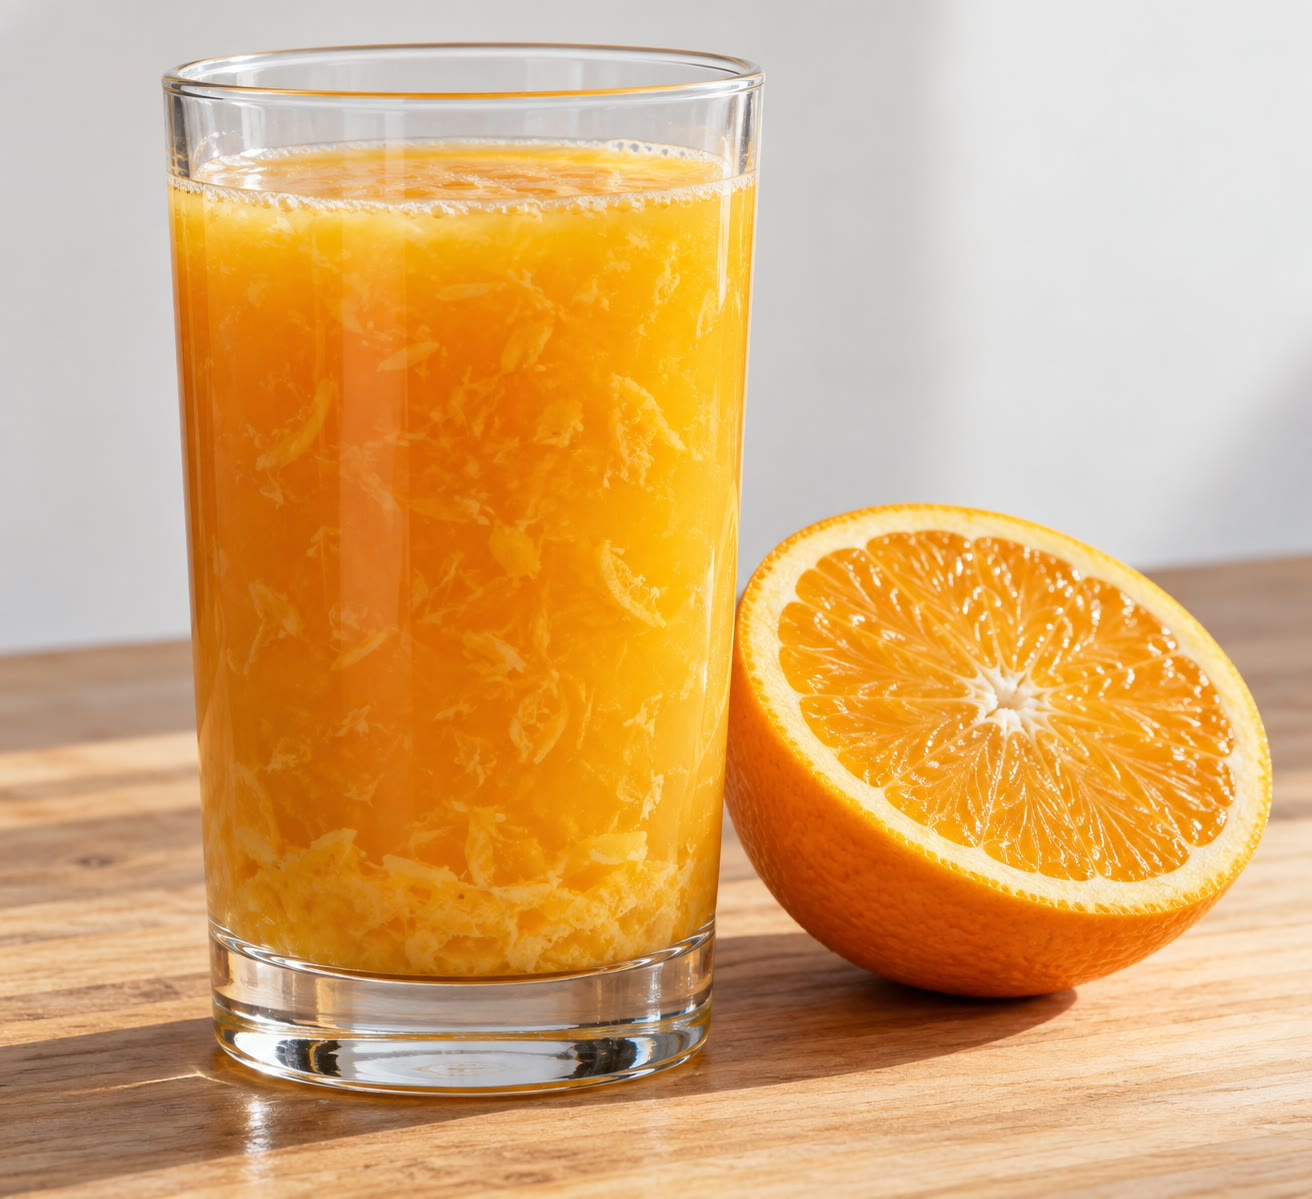
\includegraphics[width=\linewidth,height=4.6cm,keepaspectratio]{images/book1/ai/g6-orange-juice.jpg}

{\small Jus jeruk dengan bulir: sebuah \omterm{def:g6:pure-substances-and-mixtures:homogeneous}{campuran heterogen}.}
\end{minipage}
\end{omfigure}

\begin{remark}[Homogen tidak berarti murni]\label{rem:g6:pure-substances-and-mixtures:not-pure}
Air asin tampak persis seperti air murni. Melihat saja tidak cukup untuk
membedakan \omterm{def:g6:pure-substances-and-mixtures:pure-substance}{zat murni} dari \omterm{def:g6:pure-substances-and-mixtures:homogeneous}{campuran homogen}: kita harus mengukur
sesuatu.
\end{remark}

\section{Mengenali zat murni dari tetapannya}

\begin{proposition}[Zat murni memiliki tetapan sendiri]\label{prop:g6:pure-substances-and-mixtures:constants}
% ledger: mp:water, bp:water, bp:ethanol, mp:ethanol, rho:water, rho:ethanol, mp:NaCl, mp:Fe, rho:Fe
Setiap \omterm{def:g6:pure-substances-and-mixtures:pure-substance}{zat murni} mencair pada suhu tetapnya sendiri, mendidih pada suhu
tetapnya sendiri (pada tekanan normal), dan memiliki massa sendiri untuk
volume tertentu, yaitu massa jenisnya. Bilangan-bilangan itu adalah
tetapannya; buku fisika menjelaskan apa yang diukurnya. Untuk beberapa
\omterm{def:g6:pure-substances-and-mixtures:pure-substance}{zat murni}:
\begin{center}
\small
\begin{tabular}{lccc}
\hline
\omterm{def:g6:pure-substances-and-mixtures:pure-substance}{zat murni} & mencair pada & mendidih pada & massa \qty{1}{cm^3} \\
\hline
air & \qty{0}{\celsius} & \qty{100}{\celsius} & sekitar \qty{1.0}{g} \\
etanol & \qty{-114}{\celsius} & \qty{78}{\celsius} & \qty{0.79}{g} \\
propanon (aseton) & --- & \qty{56}{\celsius} & \qty{0.78}{g} \\
garam (natrium klorida) & \qty{801}{\celsius} & --- & \qty{2.17}{g} \\
besi & \qty{1538}{\celsius} & --- & \qty{7.87}{g} \\
\hline
\end{tabular}
\end{center}
% ledger: bp:acetone, rho:acetone, rho:NaCl
\end{proposition}

\begin{proposition}[Campuran tidak memiliki suhu didih tetap]\label{prop:g6:pure-substances-and-mixtures:mixture-boils}
Sebuah \omterm{def:g6:pure-substances-and-mixtures:mixture}{campuran} tidak mendidih pada satu suhu tetap: air asin mulai
mendidih sedikit di atas \qty{100}{\celsius}, dan suhunya terus naik
selama mendidih, karena airnya pergi dan garam yang tertinggal menjadi
makin pekat.
\end{proposition}

\begin{method}[Murnikah cairan ini? Cairan apakah itu?]\label{met:g6:pure-substances-and-mixtures:identify}
\begin{enumerate}
  \item Panaskan cairan itu, di laboratorium, dan baca suhunya selama
        mendidih.
  \item Jika suhunya tetap, cairan itu kemungkinan \omterm{def:g6:pure-substances-and-mixtures:pure-substance}{zat murni}:
        bandingkan suhu itu dengan tabel tetapan.
  \item Jika suhunya terus naik, cairan itu \omterm{def:g6:pure-substances-and-mixtures:mixture}{campuran}.
  \item Pastikan dengan tetapan kedua, misalnya massa suatu volume yang
        diketahui.
\end{enumerate}
\end{method}

\begin{inthelab}[Mendidihkan air asin]
Guru memanaskan air murni dan air asin berdampingan, masing-masing
dengan termometer di dalamnya. Air murni mendidih pada
\qty{100}{\celsius} dan tetap di suhu itu selama mendidih. Air asin
mulai mendidih sedikit di atas \qty{100}{\celsius}, dan termometernya
merayap naik dari menit ke menit.
\end{inthelab}

\section{Air, murni dan tidak murni}

\begin{example}[Empat macam air]\label{ex:g6:pure-substances-and-mixtures:waters}
% ledger: sea:salinity
\begin{itemize}
  \item \textbf{Air suling}, yang dibuat di laboratorium, hampir
        merupakan \omterm{def:g6:pure-substances-and-mixtures:pure-substance}{zat murni}: air dan tidak ada yang lain.
  \item \textbf{Air keran} adalah \omterm{def:g6:pure-substances-and-mixtures:homogeneous}{campuran homogen}: air dengan sedikit
        zat terlarut (setetes air yang mengering di piring gelap
        meninggalkan cincin putih).
  \item \textbf{Air mineral} adalah \omterm{def:g6:pure-substances-and-mixtures:homogeneous}{campuran homogen} yang labelnya
        mencantumkan zat-zat terlarut, dalam miligram per liter.
  \item \textbf{Air laut} adalah \omterm{def:g6:pure-substances-and-mixtures:homogeneous}{campuran homogen} yang mengandung sekitar
        \qty{35}{g} garam-garam dalam setiap kilogram.
\end{itemize}
\end{example}

\begin{omfigure}
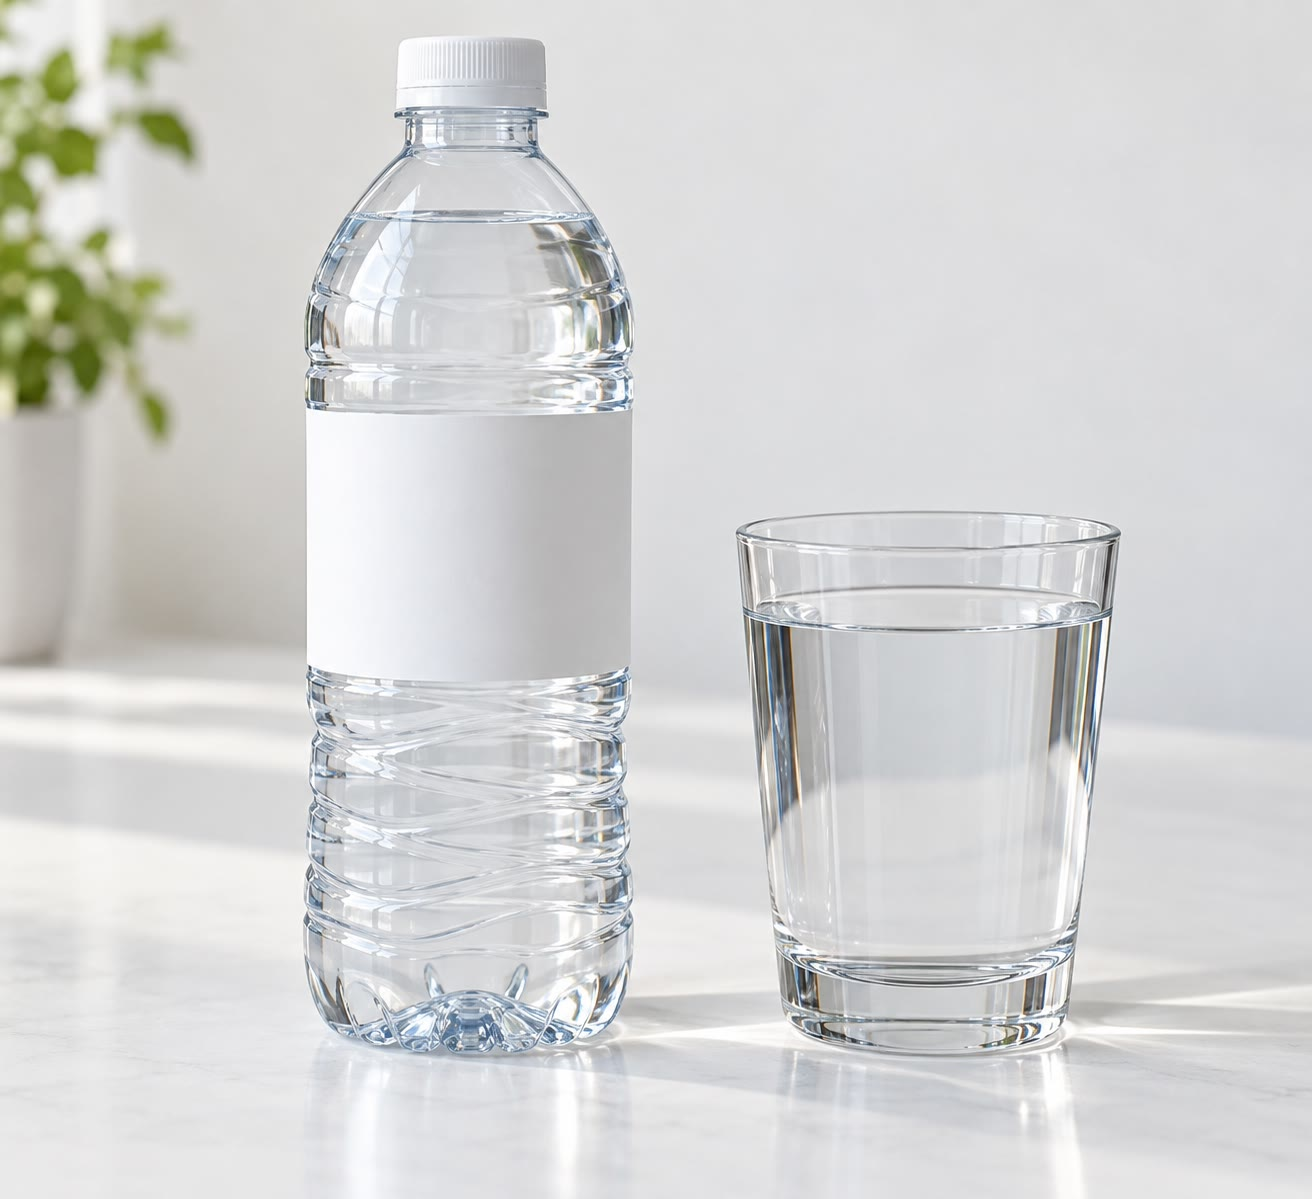
\includegraphics[width=0.5\linewidth]{images/book1/ai/g6-mineral-water.jpg}

{\small Sebotol air mineral: jernih dan tak berwarna, tetapi tetap
\omterm{def:g6:pure-substances-and-mixtures:mixture}{campuran}.}
\end{omfigure}

\begin{example}[Membaca label air mineral]\label{ex:g6:pure-substances-and-mixtures:label}
Sebuah label berbunyi: kalsium \qty{78}{mg/L}, magnesium \qty{24}{mg/L},
natrium \qty{5}{mg/L}, hidrogenkarbonat \qty{357}{mg/L}, sulfat
\qty{10}{mg/L}, klorida \qty{4}{mg/L}. (Angka-angka ini hanya contoh.)
Dalam satu liter terdapat $78 + 24 + 5 + 357 + 10 + 4 = 478$\,mg zat
terlarut, kira-kira setengah gram: sangat kecil dibandingkan
\qty{1000}{g} airnya, tetapi cukup untuk menjadikannya \omterm{def:g6:pure-substances-and-mixtures:mixture}{campuran}.
\end{example}

\section{Latihan}

\begin{exercise}[$\star$]\label{exo:g6:pure-substances-and-mixtures:1}
\omterm{def:g6:pure-substances-and-mixtures:pure-substance}{Zat murni} atau \omterm{def:g6:pure-substances-and-mixtures:mixture}{campuran}? Air suling, \omterm{def:g4:air-a-mixture-of-gases:air}{udara}, air laut, sebatang besi
murni, susu, sebutir kristal gula.
\end{exercise}

\begin{exercise}[$\star$]\label{exo:g6:pure-substances-and-mixtures:2}
Homogen atau heterogen? Air asin, granit, minyak di atas air, air
keran, muesli.
\end{exercise}

\begin{exercise}[$\star$]\label{exo:g6:pure-substances-and-mixtures:3}
Apa itu \omterm{def:g6:pure-substances-and-mixtures:species}{spesies kimia}? Berikan tiga contoh.
\end{exercise}

\begin{exercise}[$\star$]\label{exo:g6:pure-substances-and-mixtures:4}
Sebuah cairan mendidih pada \qty{78}{\celsius}, dan suhunya tetap
\qty{78}{\celsius} selama mendidih. Pakailah tabel tetapan untuk
menduga cairan apa itu.
\end{exercise}

\begin{exercise}[$\star$]\label{exo:g6:pure-substances-and-mixtures:5}
Mengapa ``jus jeruk murni'' bukan \omterm{def:g6:pure-substances-and-mixtures:pure-substance}{zat murni} bagi ahli kimia?
\end{exercise}

\begin{exercise}[$\star\star$]\label{exo:g6:pure-substances-and-mixtures:6}
Sebuah cairan mulai mendidih pada \qty{100.5}{\celsius} dan suhunya
naik selama mendidih. Apakah cairan itu \omterm{def:g6:pure-substances-and-mixtures:pure-substance}{zat murni}? Kira-kira cairan apa
itu?
\end{exercise}

\begin{exercise}[$\star\star$]\label{exo:g6:pure-substances-and-mixtures:7}
Lihatlah gambar empat gelas kimia. Di gelas kimia mana saringan dapat
memisahkan bagian-bagian \omterm{def:g6:pure-substances-and-mixtures:mixture}{campurannya}? Di gelas mana tidak dapat?
\end{exercise}

\begin{exercise}[$\star\star$]\label{exo:g6:pure-substances-and-mixtures:8}
Sebuah kubus logam bervolume \qty{10}{cm^3} memiliki massa
\qty{78.7}{g}. Berapa massa \qty{1}{cm^3}-nya? Logam mana pada tabel
yang mungkin?
\end{exercise}

\begin{exercise}[$\star\star$]\label{exo:g6:pure-substances-and-mixtures:9}
Dengan label air mineral pada contoh, berapa persen massa zat terlarut
yang berupa hidrogenkarbonat? Bulatkan ke bilangan bulat terdekat.
\end{exercise}

\begin{exercise}[$\star\star$]\label{exo:g6:pure-substances-and-mixtures:10}
Air laut mengandung sekitar \qty{35}{g} garam-garam per kilogram.
Berapa massa garam dalam seember air laut \qty{2}{kg}? Berapa persen
massa air laut yang berupa garam?
\end{exercise}

\begin{exercise}[$\star\star\star$]\label{exo:g6:pure-substances-and-mixtures:11}
Dua cairan jernih tak berwarna tampak sama persis. Uraikan dua
pengukuran, yang dilakukan di laboratorium, yang akan menunjukkan apakah
keduanya \omterm{def:g6:pure-substances-and-mixtures:pure-substance}{zat murni} yang sama.
\end{exercise}

\begin{exercise}[$\star\star\star$]\label{exo:g6:pure-substances-and-mixtures:12}
Sebuah \omterm{def:g6:pure-substances-and-mixtures:mixture}{campuran} terbuat dari \qty{90}{g} air dan \qty{10}{g} etanol.
Berapa persen massanya yang berupa etanol? Dapatkah \omterm{def:g6:pure-substances-and-mixtures:mixture}{campuran} itu
dikenali dengan tabel tetapan? Jelaskan.
\end{exercise}

\section{Soal: Tiga Cairan Tak Berwarna}

\begin{problem}[{Soal akhir pekan --- tiga labu tanpa label berisi cairan
jernih tak berwarna, dan pengukuran yang membedakannya}]
\label{pb:g6:pure-substances-and-mixtures:1}
% ledger: bp:water, bp:ethanol, rho:water, rho:ethanol, rho:seawater, sea:salinity
Seorang asisten laboratorium menemukan tiga labu, A, B, dan C, yang
labelnya terlepas. Ketiganya berisi cairan jernih tak berwarna.
Laboratorium itu hanya memakai tiga cairan semacam itu: air suling,
etanol, dan air laut yang dibawa pulang dari kunjungan lapangan. Asisten
itu melakukan tiga macam pengukuran, di laboratorium.

\medskip
\noindent\textbf{Bagian I --- Melihat.}
\begin{enumerate}
  \item Ketiga cairan tampak sama persis. Dapatkah asisten itu
        mengetahui, dengan melihat, mana yang \omterm{def:g6:pure-substances-and-mixtures:pure-substance}{zat murni}? Jelaskan.
  \item Jika salah satunya \omterm{def:g6:pure-substances-and-mixtures:mixture}{campuran}, apakah \omterm{def:g6:pure-substances-and-mixtures:mixture}{campuran} itu homogen atau
        heterogen?
  \item Pengukuran macam apa yang dapat menunjukkan bahwa sebuah cairan
        adalah \omterm{def:g6:pure-substances-and-mixtures:pure-substance}{zat murni}?
\end{enumerate}

\medskip
\noindent\textbf{Bagian II --- Mengukur.}
Setiap cairan dipanaskan sampai mendidih. Cairan A mendidih pada
\qty{100}{\celsius} dan suhunya tetap di situ. Cairan B mendidih pada
\qty{78}{\celsius} dan tetap di situ. Cairan C mulai mendidih pada
\qty{100.6}{\celsius}, dan suhunya terus naik perlahan. Lalu
\qty{50.0}{mL} dari setiap cairan ditimbang: A \qty{49.8}{g}, B
\qty{39.5}{g}, C \qty{51.2}{g}.
\begin{enumerate}[resume]
  \item Cairan mana yang \omterm{def:g6:pure-substances-and-mixtures:pure-substance}{zat murni}? Mana yang \omterm{def:g6:pure-substances-and-mixtures:mixture}{campuran}?
  \item Dengan tabel tetapan bab ini, sebutkan nama cairan A dan B.
  \item Hitung massa \qty{1}{mL} (yaitu \qty{1}{cm^3}) setiap cairan.
  \item Apakah massa-massa ini sesuai dengan jawabanmu untuk soal 5?
  \item Mengapa suhu cairan C terus naik selama mendidih?
\end{enumerate}

\medskip
\noindent\textbf{Bagian III --- Apa isi cairan C?}
\qty{100}{mL} cairan C dibiarkan mengering di dalam cawan. Ketika semua
airnya telah pergi, tersisa \qty{3.5}{g} kristal putih.
\begin{enumerate}[resume]
  \item Apa yang ditunjukkan sisa padatan ini tentang cairan C?
  \item Dengan massa \qty{1}{mL} cairan C yang diperoleh pada soal 6,
        tentukan massa \qty{100}{mL} cairan C, lalu persentase massanya
        yang berupa garam (sampai satu angka di belakang koma).
  \item Air laut mengandung sekitar \qty{35}{g} garam-garam dalam setiap
        kilogram. Berapa persen itu? Bandingkan dengan soal 10.
  \item Simpulkan: berapa gram garam yang terkandung dalam setiap liter
        cairan C, dan apakah cairan C itu air laut?
\end{enumerate}
\end{problem}
